\documentclass[a4paper,landscape]{standalone}
\usepackage{tikz}
\usetikzlibrary{arrows.meta,positioning,calc}
\usepackage{adjustbox}
\usepackage{xcolor}
\usepackage{lmodern}
\begin{document}

\begin{adjustbox}{max width=0.96\linewidth, max totalheight=0.78\textheight, center}
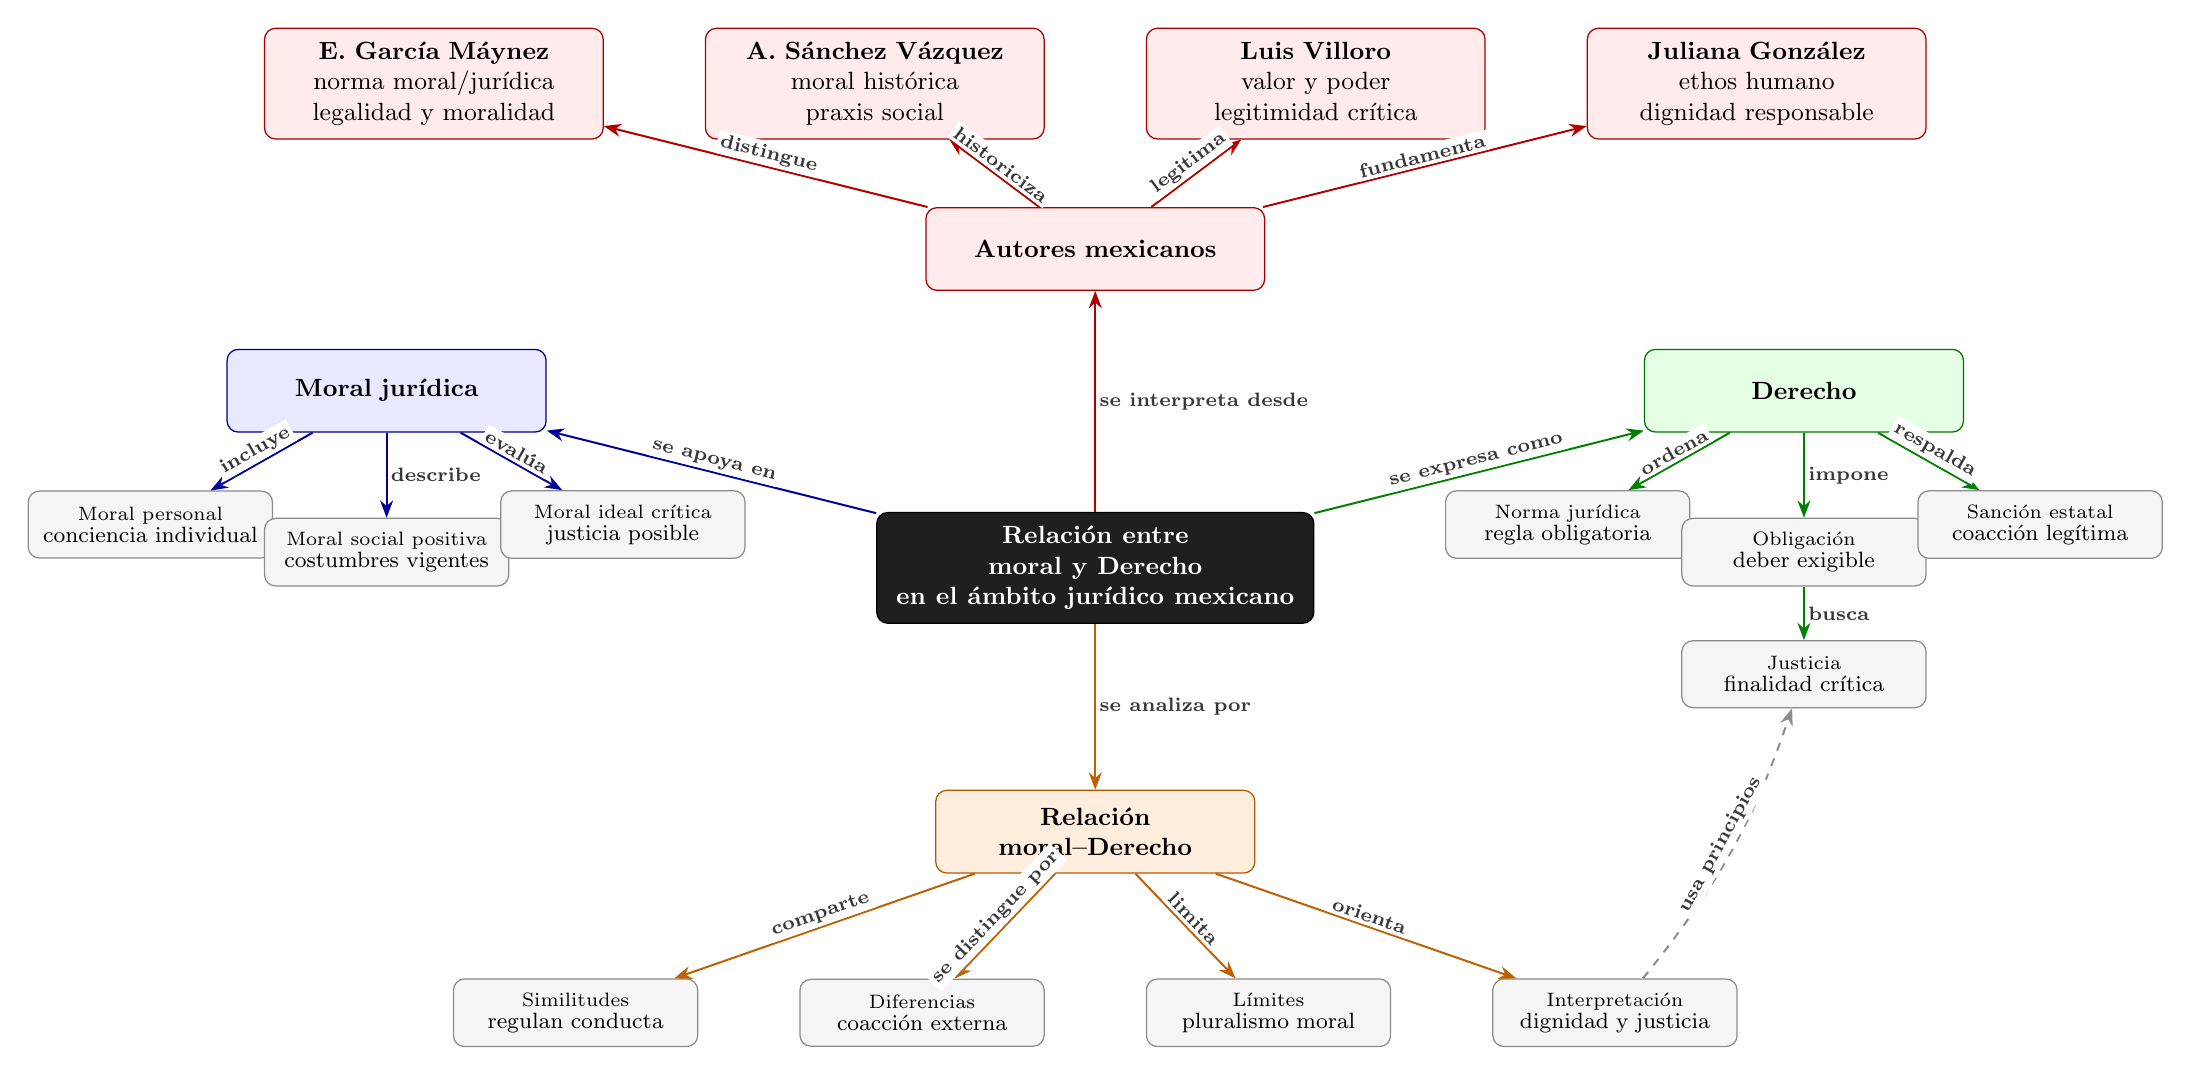
\begin{tikzpicture}[
	concept/.style={
		rectangle,
		rounded corners=4pt,
		draw=black!55,
		line width=0.45pt,
		align=center,
		text width=3.7cm,
		minimum height=1.05cm,
		inner sep=5pt,
		font=\small
	},
	root/.style={
		concept,
		fill=black!88,
		text=white,
		draw=black,
		text width=5.2cm,
		font=\bfseries\small,
		minimum height=1.35cm
	},
	moral/.style={concept, fill=blue!9, draw=blue!55!black},
	derecho/.style={concept, fill=green!10, draw=green!45!black},
	relacion/.style={concept, fill=orange!13, draw=orange!70!black},
	autor/.style={concept, fill=red!8, draw=red!65!black, text width=3.95cm},
	criterio/.style={concept, fill=gray!8, draw=black!45, text width=2.75cm, font=\scriptsize, minimum height=0.85cm},
	edge/.style={-{Stealth[length=2.2mm]}, line width=0.72pt, draw=black!60},
	label/.style={font=\scriptsize\bfseries, fill=white, inner sep=1.2pt, text=black!78}
]

\node[root] (centro) at (0,0) {Relación entre moral y Derecho\\en el ámbito jurídico mexicano};

% Ramas principales
\node[moral] (moral) at (-9,2.25) {\textbf{Moral jurídica}};
\node[derecho] (derecho) at (9,2.25) {\textbf{Derecho}};
\node[relacion] (rel) at (0,-3.35) {\textbf{Relación moral--Derecho}};
\node[autor] (autores) at (0,4.05) {\textbf{Autores mexicanos}};

\draw[edge, blue!60!black] (centro) -- node[label, above, sloped] {se apoya en} (moral);
\draw[edge, green!50!black] (centro) -- node[label, above, sloped] {se expresa como} (derecho);
\draw[edge, orange!75!black] (centro) -- node[label, right] {se analiza por} (rel);
\draw[edge, red!70!black] (centro) -- node[label, right] {se interpreta desde} (autores);

% Moral
\node[criterio] (mp) at (-12,0.55) {Moral personal\\\footnotesize conciencia individual};
\node[criterio] (msp) at (-9,0.2) {Moral social positiva\\\footnotesize costumbres vigentes};
\node[criterio] (mic) at (-6,0.55) {Moral ideal crítica\\\footnotesize justicia posible};

\draw[edge, blue!60!black] (moral) -- node[label, above, sloped] {incluye} (mp);
\draw[edge, blue!60!black] (moral) -- node[label, right] {describe} (msp);
\draw[edge, blue!60!black] (moral) -- node[label, above, sloped] {evalúa} (mic);

% Derecho
\node[criterio] (norma) at (6,0.55) {Norma jurídica\\\footnotesize regla obligatoria};
\node[criterio] (oblig) at (9,0.2) {Obligación\\\footnotesize deber exigible};
\node[criterio] (sancion) at (12,0.55) {Sanción estatal\\\footnotesize coacción legítima};
\node[criterio] (justicia) at (9,-1.35) {Justicia\\\footnotesize finalidad crítica};

\draw[edge, green!50!black] (derecho) -- node[label, above, sloped] {ordena} (norma);
\draw[edge, green!50!black] (derecho) -- node[label, right] {impone} (oblig);
\draw[edge, green!50!black] (derecho) -- node[label, above, sloped] {respalda} (sancion);
\draw[edge, green!50!black] (oblig) -- node[label, right] {busca} (justicia);

% Relaciones
\node[criterio] (sim) at (-6.6,-5.65) {Similitudes\\\footnotesize regulan conducta};
\node[criterio] (dif) at (-2.2,-5.65) {Diferencias\\\footnotesize coacción externa};
\node[criterio] (lim) at (2.2,-5.65) {Límites\\\footnotesize pluralismo moral};
\node[criterio] (interp) at (6.6,-5.65) {Interpretación\\\footnotesize dignidad y justicia};

\draw[edge, orange!75!black] (rel) -- node[label, above, sloped] {comparte} (sim);
\draw[edge, orange!75!black] (rel) -- node[label, above, sloped] {se distingue por} (dif);
\draw[edge, orange!75!black] (rel) -- node[label, above, sloped] {limita} (lim);
\draw[edge, orange!75!black] (rel) -- node[label, above, sloped] {orienta} (interp);
\draw[edge, black!45, dashed, bend right=10] (interp) to node[label, above, sloped] {usa principios} (justicia);

% Autores
\node[autor] (gm) at (-8.4,6.15) {\textbf{E. García Máynez}\\norma moral/jurídica\\legalidad y moralidad};
\node[autor] (sv) at (-2.8,6.15) {\textbf{A. Sánchez Vázquez}\\moral histórica\\praxis social};
\node[autor] (lv) at (2.8,6.15) {\textbf{Luis Villoro}\\valor y poder\\legitimidad crítica};
\node[autor] (jg) at (8.4,6.15) {\textbf{Juliana González}\\ethos humano\\dignidad responsable};

\draw[edge, red!70!black] (autores) -- node[label, above, sloped] {distingue} (gm);
\draw[edge, red!70!black] (autores) -- node[label, above, sloped] {historiciza} (sv);
\draw[edge, red!70!black] (autores) -- node[label, above, sloped] {legitima} (lv);
\draw[edge, red!70!black] (autores) -- node[label, above, sloped] {fundamenta} (jg);

\end{tikzpicture}
\end{adjustbox}

\end{document}
